% MedTwin paper -- Springer LNCS format.
% Build on Overleaf (New Project > Templates > "Springer Lecture Notes in
% Computer Science") or locally with llncs.cls and splncs04.bst next to
% this file:  pdflatex main && bibtex main && pdflatex main && pdflatex main
% Tables in tables/ are generated by research/paper_tables.py; figures in
% figures/ are copied from ../figures (research/visualizer.py).
\documentclass[runningheads]{llncs}

\usepackage[T1]{fontenc}
\usepackage{graphicx}
\usepackage{booktabs}
\usepackage{amsmath}
\usepackage{amssymb}
\usepackage{url}
\usepackage[hidelinks]{hyperref}

\graphicspath{{figures/}}

\begin{document}

\title{Missingness-Aware Conditional WGAN-GP for Synthetic Multi-Site Clinical Records}
\titlerunning{Missingness-Aware Synthetic Clinical Records}

\author{Aarzoo Jain \and Pranav Ladha}
\authorrunning{A. Jain and P. Ladha}
\institute{Department of Data Science and Engineering, Manipal University Jaipur, Jaipur, India\\
\email{aarzoo.23fe10cds00459@muj.manipal.edu}, \email{pranav.23fe10cds00455@muj.manipal.edu}}

\maketitle

\begin{abstract}
Synthetic patient records are a promising way to share clinical data
without exposing real patients, but real clinical tables are incomplete in
structured ways: whether a test was performed often depends on the hospital
that recorded it. Common tabular generators either require complete data or
fill gaps before training, so the synthetic cohort loses this structure. We
present MedTwin, a conditional Wasserstein GAN with gradient penalty that
treats ``not measured'' as part of the record: it generates a measurement
flag for every incompletely observed column, a separate flag for values with
a large spike at exactly zero, and conditions each record on its site. We
evaluate on the four-site UCI heart disease data (920 patients) and the Pima
diabetes data (768 patients) against CTGAN, TVAE and TabDDPM, using five
seeds with held-out patients and paired confidence intervals. MedTwin gives
the highest histogram fidelity on both datasets and the least detectable
records on heart disease (61.5\% real-vs-synthetic classifier accuracy
against 74.9--92.8\% for the baselines), with downstream utility matching
the best baseline (TSTR/TRTR AUC ratio 0.975 and 0.983). Membership
inference and distance-to-closest-record tests show no detectable
memorisation, unlike TabDDPM on diabetes (membership-inference AUC 0.80).
Ablations show that the measurement flags, the zero flag and site
conditioning each make records clearly harder to detect, while a
correlation-matching loss leaves realism and utility unchanged but roughly
halves the gap between real and synthetic correlations of numeric columns
(0.075 to 0.041 on heart disease, 0.063 to 0.034 on diabetes).
\keywords{Synthetic data \and Generative adversarial networks \and Missing data \and Electronic health records \and Privacy evaluation}
\end{abstract}

% ---------------------------------------------------------------------------
\section{Introduction}

Machine learning for clinical prediction depends on access to patient data
that privacy law and institutional policy rightly restrict. Synthetic data
--- records drawn from a generative model trained on real patients --- is
one proposed way to share such data, and tabular generators such as
CTGAN~\cite{xu2019ctgan}, TVAE~\cite{xu2019ctgan} and
TabDDPM~\cite{kotelnikov2023tabddpm} are now standard tools for it.

Clinical tables, however, are rarely complete, and their gaps are not
random. In the UCI heart disease data, collected at four hospitals for
Detrano et al.~\cite{detrano1989}, every Swiss patient has a serum
cholesterol of 0 (the test was not recorded), the number of major vessels
coloured by fluoroscopy is missing for 96--99\% of patients at three of the
four sites, and resting blood pressure is missing for 28\% of VA Long Beach
patients but almost no one elsewhere. A faithful synthetic version of this
cohort must reproduce \emph{which} tests were performed \emph{where}. Yet
most tabular generators require complete input, so missing values are
usually imputed first, and the generated cohort then contains invented
measurements that no real record had.

We present MedTwin, a conditional WGAN-GP~\cite{gulrajani2017wgangp} for
mixed-type clinical tables that generates missingness instead of removing
it. Our contributions are:
\begin{enumerate}
\item \textbf{Site-conditioned missingness for small multi-site tables.}
  Building on recent work that preserves missingness in synthetic
  data~\cite{bing2022healthgen,ouyang2023missdiff,wang2025reinvented}, we
  use a deliberately simple mechanism suited to small tables: each
  incompletely observed numeric column gets a generated ``measured'' flag,
  missing categories are a category of their own, zeros that encode
  ``not measured'' are recognised from the dataset's settings, and the
  flags are generated conditionally on the site.
\item \textbf{Site conditioning and zero-spike flags.} Records are generated
  for a given hospital, so site-specific measurement practice is learned,
  and a binary flag reproduces the large point mass at zero of ST
  depression (40\% of patients).
\item \textbf{A held-out evaluation that separates realism from privacy.}
  We report utility (train-on-synthetic, test-on-real), realism
  (fidelity, real-vs-synthetic \emph{detectability}) and privacy
  (distance to closest record, membership inference) against patients
  never seen in training, and argue that detectability, sometimes reported
  as a privacy score, is not one.
\item \textbf{A five-seed benchmark with ablations.} On two datasets we
  compare against CTGAN, TVAE and TabDDPM under identical preprocessing and
  scoring, ablate each component, and test sensitivity to the main
  hyperparameters, with paired confidence intervals throughout.
\end{enumerate}

% ---------------------------------------------------------------------------
\section{Related Work}

\paragraph{Tabular and health-record generators.}
medGAN~\cite{choi2017medgan} generated high-dimensional binary and count
EHR features. CTGAN~\cite{xu2019ctgan} handled mixed-type tables with
mode-specific normalisation and a conditional generator trained by
sampling; the same work proposed TVAE. CTAB-GAN~\cite{zhao2021ctabgan}
extended this to mixed and long-tailed variables. Diffusion models now lead
general tabular benchmarks: TabDDPM~\cite{kotelnikov2023tabddpm} combines
Gaussian and multinomial diffusion, and TabSyn~\cite{zhang2024tabsyn} runs
score-based diffusion in a learned latent space. For real EHRs,
EHR-Safe~\cite{yoon2023ehrsafe} addresses heterogeneity, sparsity and
variable-length sequences. MedTwin builds on WGAN-GP~\cite{gulrajani2017wgangp}
with Gumbel-softmax categorical outputs~\cite{jang2017gumbel}.

\paragraph{Missing data.}
GAIN~\cite{yoon2018gain} imputes missing entries adversarially, with a
discriminator that guesses which entries were observed.
MisGAN~\cite{li2019misgan} learns a mask generator alongside the data
generator so that the missingness pattern is itself modelled. More recent
work makes the synthetic records themselves incomplete. HealthGen~\cite{bing2022healthgen} generates medical time series that keep their
informative missingness; MissDiff~\cite{ouyang2023missdiff} trains
diffusion models directly on incomplete tables and shows that
``impute-then-generate'' biases the learned distribution; Wang et
al.~\cite{wang2025reinvented} preserve both the observed and the missing
data distributions in a way that plugs into existing generators;
IGAMT~\cite{wang2024igamt} handles missing and irregular EHR measurements
under differential privacy; and Petrakos et al.~\cite{petrakos2025rct}
add missingness models to synthetic trial data. MedTwin shares their goal.
It differs in using an explicit site condition for missingness that is
driven by hospital practice, in a simple flag encoding that also works for
zero-coded gaps, and in a controlled ablation of that encoding against
imputation under a multi-seed held-out protocol.

\paragraph{Evaluation.}
Train-on-synthetic, test-on-real (TSTR) was introduced for medical time
series by Esteban et al.~\cite{esteban2017rcgan}. Alaa et
al.~\cite{alaa2022faithful} separate fidelity, diversity and generalisation
(not copying training records). Distance to closest record is a common
privacy check~\cite{zhao2021ctabgan}, and membership inference attacks on
generative models were shown by LOGAN~\cite{hayes2019logan} and
systematised by GAN-Leaks~\cite{chen2020ganleaks}. Stadler et
al.~\cite{stadler2022groundhog} show that synthetic data does not, in
general, offer a better privacy--utility trade-off than traditional
anonymisation, so empirical privacy checks must not be read as guarantees.
Synthcity~\cite{qian2023synthcity} collects generators and metrics in one
benchmark framework.

% ---------------------------------------------------------------------------
\section{Method}

\subsection{Encoding records with their missingness}
\label{sec:encoding}

Each dataset is described by a settings file listing its numeric and
categorical columns, the columns in which 0 means ``not measured'', the
columns with a spike at exactly zero, an optional condition column (the
site), and plausible clinical ranges. A real record $r$ is encoded as
follows.

\emph{Not-measured values.} Zeros in the listed columns become missing.
Every numeric column $j$ that is missing for at least one patient receives
a flag $m_j = 1$ if it was not measured; its value is replaced by the
training median as a placeholder that the flag marks as meaningless.

\emph{Zero spikes.} A Sigmoid output cannot place a point mass on one exact
value, so for each listed column we add a flag $z_j = \mathbb{1}[x_j = 0]$.

\emph{Scaling and categories.} Numeric values are min--max scaled to
$[0,1]$, matching the Sigmoid outputs of the generator. Each categorical
column is one-hot encoded, with ``not measured'' as an extra category.

\emph{Condition.} The site is not generated; it is a one-hot condition
vector $c$. Datasets without a site column use a constant condition, which
reduces the model to an unconditional GAN.

\subsection{Conditional WGAN-GP}

The generator $G(z, c)$ maps noise $z \sim \mathcal{N}(0, I_{128})$ and the
condition through two hidden layers (256 and 512 units, LeakyReLU, batch
normalisation). Its output is split into segments: one Sigmoid segment for
scaled numerics and all flags, and one Gumbel-softmax
segment~\cite{jang2017gumbel} (temperature $\tau = 0.2$) per categorical
column, which is relaxed during training and exactly one-hot when sampling.
The critic $D(x, c)$ scores a record together with its condition (layers of
512 and 256 units, LeakyReLU, dropout 0.3), so it judges whether a record is
realistic \emph{for that site}. Training follows WGAN-GP:
\begin{equation}
\mathcal{L}_D = \mathbb{E}[D(\tilde{x}, c)] - \mathbb{E}[D(x, c)]
  + \lambda\, \mathbb{E}\big[(\lVert \nabla_{\hat{x}} D(\hat{x}, c) \rVert_2 - 1)^2\big],
\end{equation}
with $\tilde{x} = G(z, c)$ generated for the same sites as the real batch,
$\hat{x}$ interpolated between real and generated records at fixed $c$, and
$\lambda = 10$. The generator loss adds a correlation-matching term,
\begin{equation}
\mathcal{L}_G = -\mathbb{E}[D(\tilde{x}, c)]
  + \alpha\, \big\lVert \mathrm{corr}([x, c]) - \mathrm{corr}([\tilde{x}, c]) \big\rVert_F^2 / d^2,
\end{equation}
the mean squared difference between the Pearson correlation matrices of the
real and generated batch (including the condition), with $\alpha = 2$.
Columns that are constant within a batch have no defined correlation and
are excluded; without this, a batch that happens to contain no patients of
a rare category produces NaN gradients that corrupt training.

We train for 600 epochs with batch size 64, five critic updates per
generator update, and Adam (learning rate $10^{-4}$,
$\beta = (0, 0.9)$).

\subsection{Decoding}

To sample $n$ records we draw sites with their training frequencies, so
site proportions match the real data exactly. Numeric outputs are mapped
back to clinical units; a zero flag $\geq 0.5$ sets the value to 0, and a
measurement flag $\geq 0.5$ blanks it (``not measured'' takes precedence).
Records outside the plausible clinical ranges are removed --- ranges chosen
to include every measured real value, so no real patient would be
filtered --- and values are rounded to their recorded precision (e.g.\ ST
depression to 0.1), with counts and scores clipped to their ranges.

% ---------------------------------------------------------------------------
\section{Experimental Setup}

\paragraph{Datasets.}
\emph{Heart disease} (UCI) has 920 patients from Cleveland (304), Hungary
(293), VA Long Beach (200) and Switzerland (123), with 7 numeric and 7
categorical columns plus the site; 55.3\% have disease (severity
$> 0$). Five numeric columns are sometimes missing, and missingness is
strongly site-dependent (Sect.~\ref{sec:missingness}). \emph{Pima
diabetes}~\cite{smith1988adap} has 768 patients with 9 numeric columns and
no site; zeros in glucose, blood pressure, skin fold, insulin and BMI mean
``not measured'' (insulin: 48.7\% of patients), while 0 pregnancies is a
real value. Both datasets run from settings files alone, with no code
changes.

\paragraph{Protocol.}
For each of five seeds, 20\% of patients are held out (stratified on the
outcome) and never seen by any generator; the seed also sets every model's
initialisation. Each model generates 2000 records, which pass through the
same plausibility filter and rounding. We report mean $\pm$ SD over seeds
and compare models seed-by-seed with paired $t$-based 95\% confidence
intervals; a difference is called \emph{clear} when its interval excludes
zero.

\paragraph{Baselines.}
CTGAN and TVAE~\cite{xu2019ctgan} (300 epochs, batch size 100) and TabDDPM
(8000 steps), the last a compact reimplementation of the published
design~\cite{kotelnikov2023tabddpm}. None accepts missing values, so they
receive the same measurement-flag and placeholder encoding as MedTwin and
their flagged values are blanked in the same way; they are unconditional
and generate the site like any other column.

\paragraph{Metrics.}
\emph{Fidelity}: mean histogram overlap (20 bins) between real and
synthetic distributions of four key numeric columns, on measured values.
\emph{Detectability}: held-out accuracy of a random forest trained to tell
real from synthetic records on a balanced sample (50\% = indistinguishable).
\emph{Utility}: a random forest trained on synthetic (TSTR) or real
training (TRTR) records predicts the binary outcome of held-out patients; we
report TSTR AUC and the ratio TSTR/TRTR. \emph{DCR}: the share of synthetic
records whose nearest real record is a training rather than a held-out
patient, with equally sized real sets (50\% = no memorisation).
\emph{Membership inference}: AUC of an attacker who scores each real patient
by its distance to the nearest synthetic record (0.5 = no leakage).
\emph{Correlation gap}: mean absolute difference between the real
(training) and synthetic Pearson correlation matrices, over all encoded
features (numerics, flags and categories) and, more readably, between the
numeric columns only on measured values.

\paragraph{Detectability is not privacy.}
A generator that copied its training records would be undetectable. We
therefore treat detectability as a realism measure and base privacy
statements only on DCR and membership inference against held-out patients.

% ---------------------------------------------------------------------------
\section{Results}

\subsection{Comparison with baselines}

\begin{table}[t]
\caption{Heart disease, mean $\pm$ SD over five seeds (best mean in bold).
Arrows give the direction of better; $\to$ marks a target value.}
\label{tab:heart}
\centering\scriptsize\setlength{\tabcolsep}{3pt}
% Generated by research/paper_tables.py -- do not edit by hand.
\begin{tabular}{lcccccc}
\toprule
Model & Fidelity (\%) $\uparrow$ & TSTR AUC $\uparrow$ & AUC ratio $\uparrow$ & Detect. (\%) $\to 50$ & DCR (\%) $\to 50$ & MIA AUC $\to 0.5$ \\
\midrule
MedTwin (ours) & \textbf{87.5} $\pm$ 0.8 & 0.863 $\pm$ 0.023 & 0.975 $\pm$ 0.032 & \textbf{61.5} $\pm$ 1.3 & 52.9 $\pm$ 2.8 & 0.533 $\pm$ 0.030 \\
CTGAN & 74.2 $\pm$ 4.6 & 0.696 $\pm$ 0.069 & 0.787 $\pm$ 0.082 & 92.8 $\pm$ 1.6 & 51.1 $\pm$ 3.4 & \textbf{0.507} $\pm$ 0.020 \\
TVAE & 85.6 $\pm$ 1.1 & \textbf{0.873} $\pm$ 0.022 & \textbf{0.987} $\pm$ 0.024 & 79.5 $\pm$ 2.8 & \textbf{50.1} $\pm$ 3.4 & 0.531 $\pm$ 0.023 \\
TabDDPM & 86.1 $\pm$ 1.1 & 0.820 $\pm$ 0.030 & 0.926 $\pm$ 0.022 & 74.9 $\pm$ 2.8 & 52.7 $\pm$ 3.0 & 0.526 $\pm$ 0.033 \\
\bottomrule
\end{tabular}

\end{table}

\begin{table}[t]
\caption{Pima diabetes, mean $\pm$ SD over five seeds (best mean in bold).}
\label{tab:diabetes}
\centering\scriptsize\setlength{\tabcolsep}{3pt}
% Generated by research/paper_tables.py -- do not edit by hand.
\begin{tabular}{lcccccc}
\toprule
Model & Fidelity (\%) $\uparrow$ & TSTR AUC $\uparrow$ & AUC ratio $\uparrow$ & Detect. (\%) $\to 50$ & DCR (\%) $\to 50$ & MIA AUC $\to 0.5$ \\
\midrule
MedTwin (ours) & \textbf{90.9} $\pm$ 0.8 & 0.801 $\pm$ 0.030 & 0.983 $\pm$ 0.041 & 64.0 $\pm$ 2.6 & 51.8 $\pm$ 1.8 & 0.494 $\pm$ 0.021 \\
CTGAN & 77.8 $\pm$ 3.3 & 0.568 $\pm$ 0.062 & 0.697 $\pm$ 0.075 & 86.3 $\pm$ 2.7 & \textbf{49.7} $\pm$ 7.7 & \textbf{0.505} $\pm$ 0.028 \\
TVAE & 88.0 $\pm$ 1.7 & \textbf{0.806} $\pm$ 0.013 & \textbf{0.989} $\pm$ 0.028 & 70.0 $\pm$ 1.4 & 54.0 $\pm$ 2.4 & 0.518 $\pm$ 0.024 \\
TabDDPM & 85.4 $\pm$ 1.3 & 0.781 $\pm$ 0.050 & 0.957 $\pm$ 0.026 & \textbf{55.9} $\pm$ 2.6 & 60.8 $\pm$ 4.9 & 0.803 $\pm$ 0.028 \\
\bottomrule
\end{tabular}

\end{table}

Tables~\ref{tab:heart} and~\ref{tab:diabetes} summarise the benchmark and
Fig.~\ref{fig:benchmark} shows it for heart disease. On both datasets
MedTwin has the highest fidelity, clearly higher than every baseline in
paired comparisons (by 1.4--13.3 points on heart disease and 2.9--13.1 on
diabetes). On heart disease its records are also the least detectable:
61.5\% against 74.9\% for TabDDPM, 79.5\% for TVAE and 92.8\% for CTGAN,
a clear difference in every paired comparison. Utility matches the
strongest baseline: the TSTR/TRTR AUC ratio is 0.975 (heart disease) and
0.983 (diabetes), with no clear difference from TVAE (0.987, 0.989) and
clearly above CTGAN.

On diabetes, TabDDPM is the least detectable model (55.9\% against 64.0\%
for MedTwin) but memorises its training patients: 60.8\% of its records are
closer to a training than to a held-out patient, and membership inference
reaches an AUC of 0.803 (MedTwin: 51.8\% and 0.494). For MedTwin, CTGAN and
TVAE, mean DCR stays within 49.7--54.0\% and membership-inference AUC
within 0.494--0.533 on both datasets, and no model produced an exact copy
of a training record: these tests detect no memorisation. They are empirical checks against one
attacker, not a formal guarantee.

\begin{figure}[t]
\centering
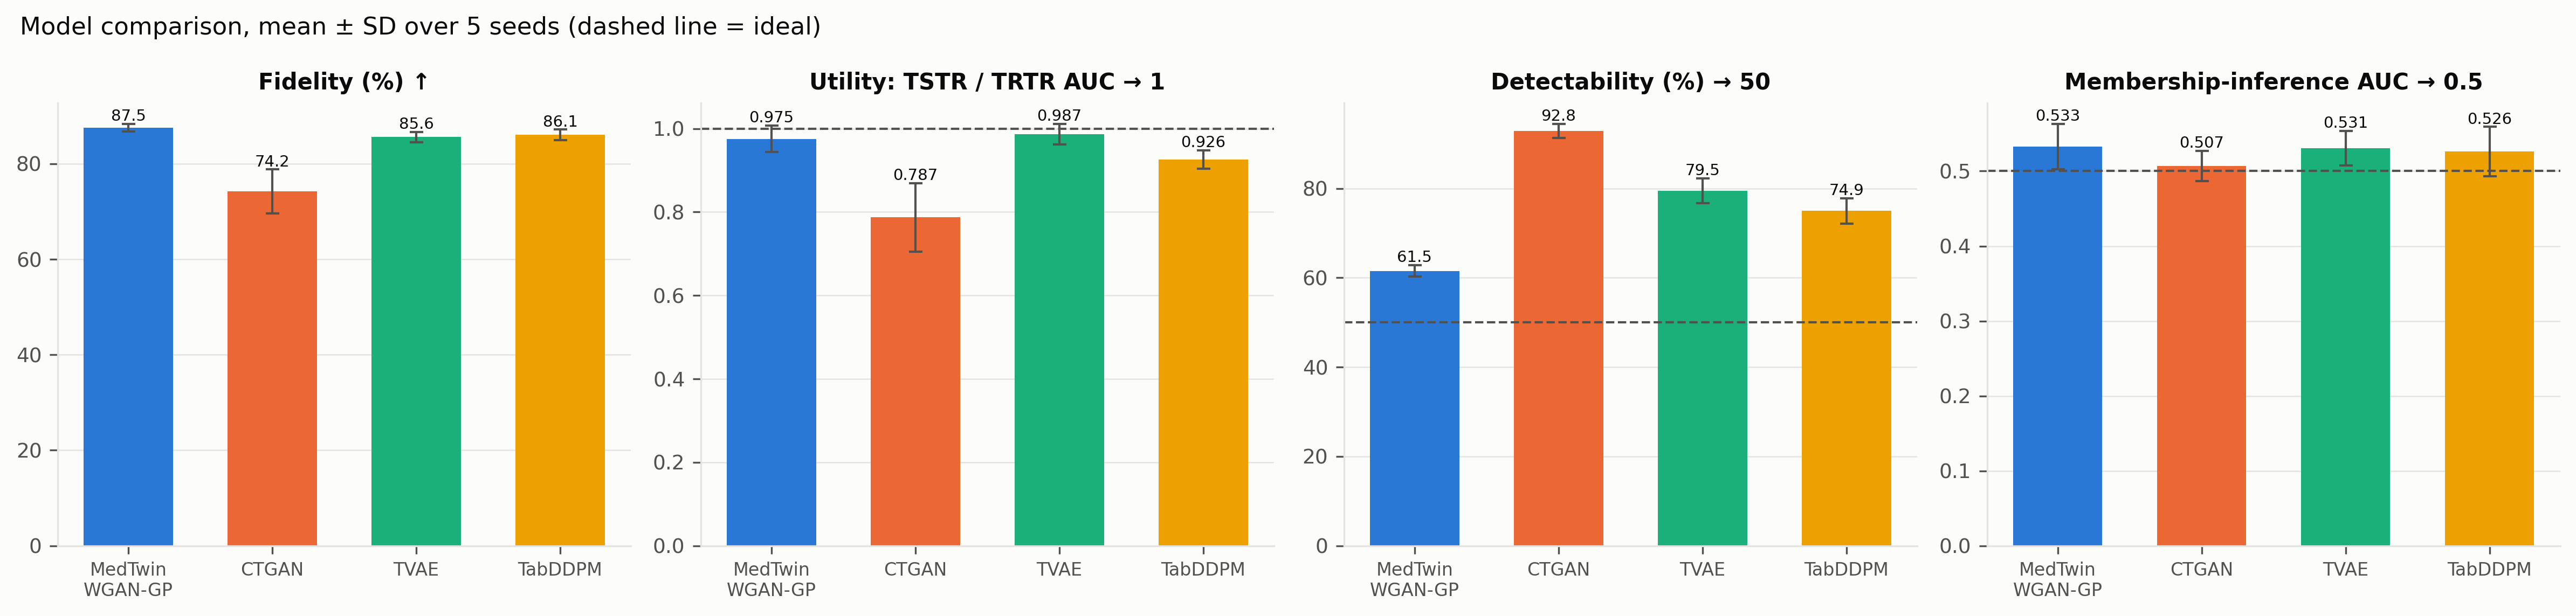
\includegraphics[width=\textwidth]{heart_disease/fig_benchmark}
\caption{Heart disease benchmark, mean $\pm$ SD over five seeds; dashed
lines mark the ideal value.}
\label{fig:benchmark}
\end{figure}

\subsection{Reproducing site-specific missingness}
\label{sec:missingness}

Fig.~\ref{fig:missingness} compares, for each site, the share of patients
with each value not measured. MedTwin reproduces the structure of the real
data: cholesterol missing for every Swiss patient and 28\% of VA patients,
vessel counts missing almost everywhere except Cleveland, and thalassemia
missing for most Hungarian and VA patients. Because each record is
generated for its site, these patterns need not be inferred from the other
columns. The largest deviations are for fasting blood sugar in Switzerland
(61\% real, 72\% synthetic), cholesterol at VA Long Beach (28\% against
35\%) and ST slope in Switzerland (14\% against 7\%).

\begin{figure}[t]
\centering
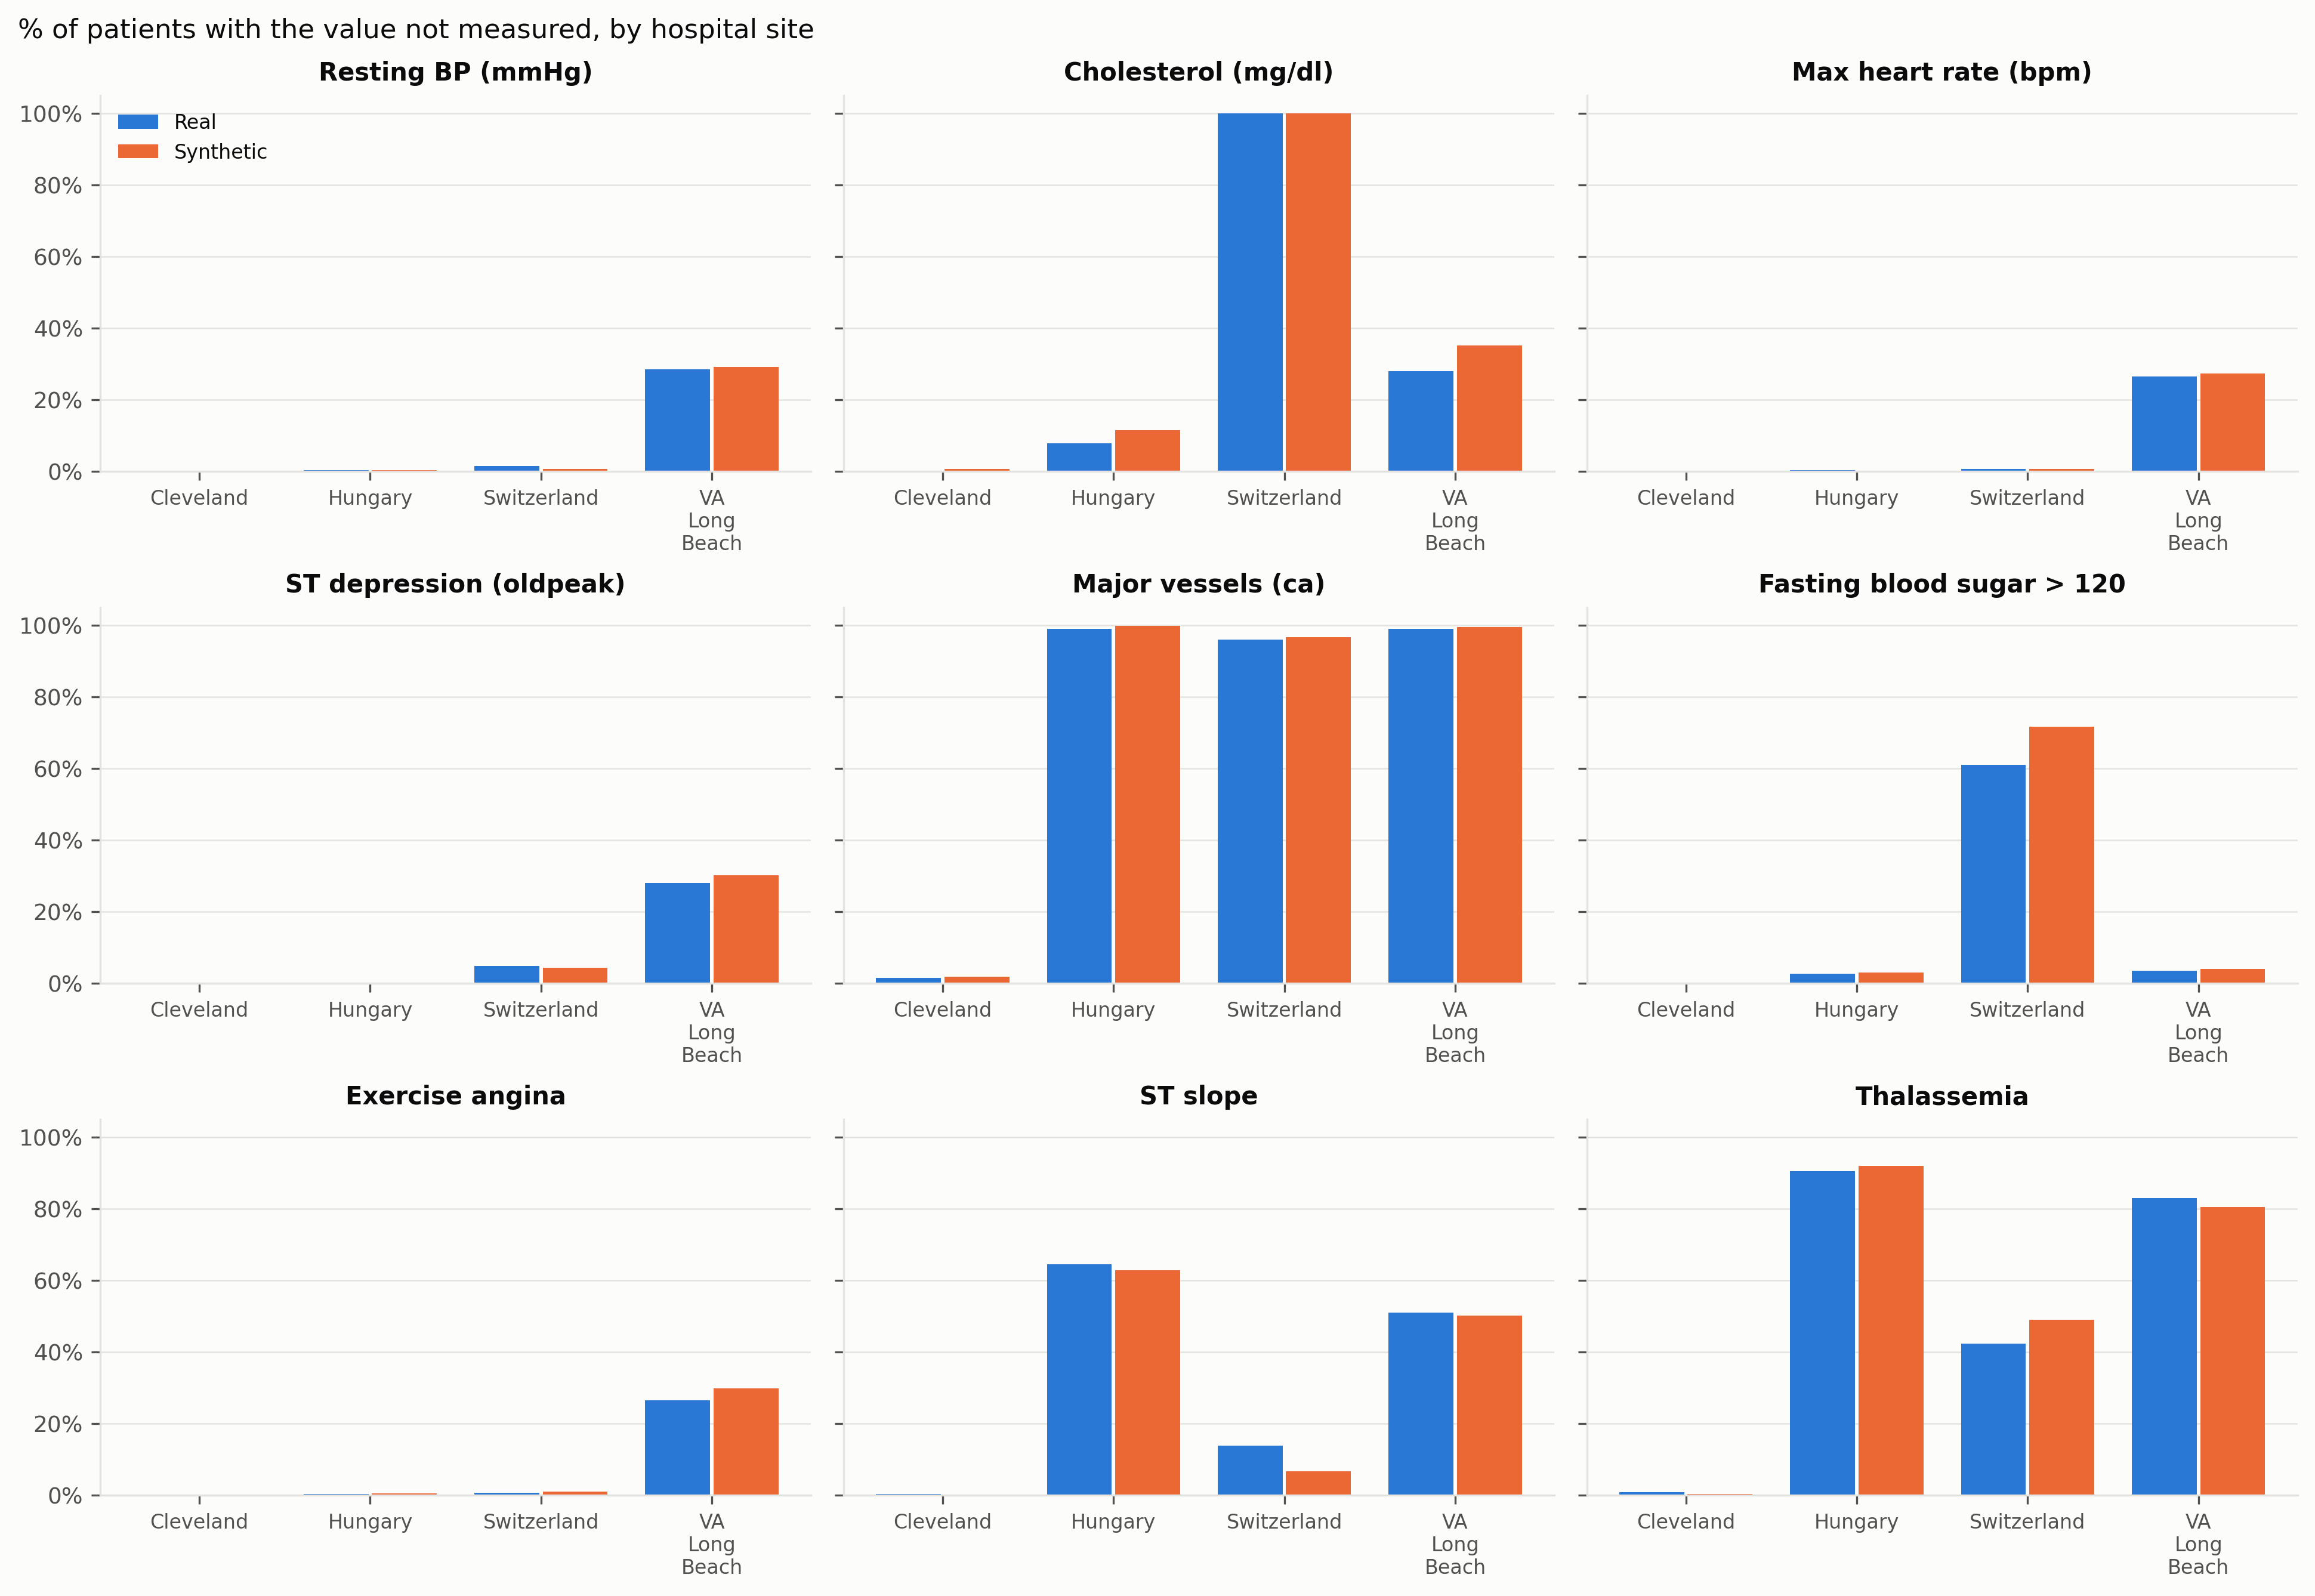
\includegraphics[width=\textwidth]{heart_disease/fig_missingness_by_site}
\caption{Share of heart disease patients with each value not measured, by
site: real (blue) and MedTwin (orange).}
\label{fig:missingness}
\end{figure}

\subsection{Ablations}

\begin{table}[t]
\caption{Ablations, mean $\pm$ SD over five seeds. Each row removes one
component from the full model; $^*$ marks a clear paired difference from
the full model (95\% CI excludes 0). Variants that do not apply to a
dataset are omitted.}
\label{tab:ablation}
\centering\scriptsize\setlength{\tabcolsep}{2.5pt}
% Generated by research/paper_tables.py -- do not edit by hand.
\begin{tabular}{lcccccc}
\toprule
Variant & Fid.\ (\%) & Detect.\ (\%) & Corr.\ gap & AUC ratio & DCR (\%) & MIA AUC \\
\midrule
\multicolumn{7}{l}{\textit{Heart disease}} \\
Full model & 87.2 $\pm$ 0.7 & 62.2 $\pm$ 1.7 & 0.025 $\pm$ 0.001 & 0.974 $\pm$ 0.028 & 53.2 $\pm$ 2.0 & 0.532 $\pm$ 0.030 \\
w/o correlation loss & 87.7 $\pm$ 0.4 & 65.2 $\pm$ 2.4 & 0.030 $\pm$ 0.003$^*$ & 0.982 $\pm$ 0.011 & 52.8 $\pm$ 2.5 & 0.525 $\pm$ 0.032 \\
w/o missing-value flags & 87.7 $\pm$ 0.2 & 84.2 $\pm$ 1.2$^*$ & 0.023 $\pm$ 0.002 & 0.989 $\pm$ 0.025 & 53.2 $\pm$ 2.6 & 0.515 $\pm$ 0.027 \\
w/o zero flag (oldpeak) & 87.1 $\pm$ 0.8 & 74.9 $\pm$ 0.9$^*$ & -- & 0.978 $\pm$ 0.032 & 53.8 $\pm$ 2.4 & 0.539 $\pm$ 0.038 \\
w/o site conditioning & 87.2 $\pm$ 0.2 & 65.6 $\pm$ 1.7$^*$ & 0.027 $\pm$ 0.002 & 0.975 $\pm$ 0.038 & 52.8 $\pm$ 2.0 & 0.527 $\pm$ 0.025 \\
\midrule
\multicolumn{7}{l}{\textit{Diabetes}} \\
Full model & 90.9 $\pm$ 0.8 & 64.0 $\pm$ 2.6 & 0.027 $\pm$ 0.003 & 0.983 $\pm$ 0.041 & 51.8 $\pm$ 1.8 & 0.494 $\pm$ 0.021 \\
w/o correlation loss & 91.0 $\pm$ 0.9 & 63.8 $\pm$ 2.9 & 0.048 $\pm$ 0.004$^*$ & 0.964 $\pm$ 0.032 & 52.0 $\pm$ 2.9 & 0.508 $\pm$ 0.029 \\
w/o missing-value flags & 88.4 $\pm$ 2.6 & 81.5 $\pm$ 1.6$^*$ & 0.038 $\pm$ 0.003$^*$ & 0.993 $\pm$ 0.032 & 52.5 $\pm$ 4.5 & 0.524 $\pm$ 0.055 \\
\bottomrule
\end{tabular}

\end{table}

Table~\ref{tab:ablation} removes one component at a time. Replacing the
measurement flags by median imputation, the usual approach, makes records
far easier to detect (heart disease 62.2\% $\to$ 84.2\%; diabetes
64.0\% $\to$ 81.5\%) while fidelity and utility change little: imputed values
blend into the marginal distributions but produce records unlike any real
patient. Removing the zero flag raises detectability on heart disease to
74.9\%, as the model can no longer place 40\% of ST depression values at
exactly zero, and removing site conditioning raises it to 65.6\%.
Removing the correlation loss changes no realism, utility or privacy
metric, but clearly worsens the correlation gap on both datasets in every
seed: between numeric columns it nearly doubles (heart disease 0.041 $\to$
0.075; diabetes 0.034 $\to$ 0.063), and over all encoded features it grows
from 0.025 to 0.030 and from 0.027 to 0.048. The loss therefore does what it
is designed to do --- preserve pairwise structure --- without trading off
anything else. No component changes utility, DCR or membership inference:
their effect is on realism (detectability and correlations), not on what
the data can be used for or on privacy.

The plausibility filter is not ablated: across all runs it removed no
record, because the Sigmoid outputs map back into the range of the training
data, which lies within the clinical ranges. It is a safeguard, not a
contributor to the results.

\subsection{Sensitivity to hyperparameters}

\begin{table}[t]
\caption{Sensitivity of the full model on heart disease to the correlation
weight $\alpha$ and the number of training epochs; $^*$ as in
Table~\ref{tab:ablation}.}
\label{tab:sensitivity}
\centering\scriptsize\setlength{\tabcolsep}{2.5pt}
% Generated by research/paper_tables.py -- do not edit by hand.
\begin{tabular}{lcccccc}
\toprule
Variant & Fid.\ (\%) & Detect.\ (\%) & Corr.\ gap & AUC ratio & DCR (\%) & MIA AUC \\
\midrule
\multicolumn{7}{l}{\textit{Heart disease}} \\
Full model & 87.2 $\pm$ 0.7 & 62.2 $\pm$ 1.7 & 0.025 $\pm$ 0.001 & 0.974 $\pm$ 0.028 & 53.2 $\pm$ 2.0 & 0.532 $\pm$ 0.030 \\
Correlation weight 0.5 (default 2) & 87.0 $\pm$ 0.8 & 62.8 $\pm$ 2.8 & -- & 0.983 $\pm$ 0.021 & 53.3 $\pm$ 2.1 & 0.531 $\pm$ 0.023 \\
Correlation weight 8 & 87.9 $\pm$ 0.5 & 62.8 $\pm$ 2.3 & -- & 0.989 $\pm$ 0.031 & 53.9 $\pm$ 2.6 & 0.525 $\pm$ 0.032 \\
300 epochs (default 600) & 87.0 $\pm$ 0.5 & 63.6 $\pm$ 2.8 & -- & 0.961 $\pm$ 0.034 & 52.2 $\pm$ 2.5 & 0.524 $\pm$ 0.035 \\
1200 epochs & 87.2 $\pm$ 0.5 & 63.0 $\pm$ 2.2 & -- & 0.984 $\pm$ 0.017 & 55.3 $\pm$ 2.6$^*$ & 0.548 $\pm$ 0.024$^*$ \\
\bottomrule
\end{tabular}

\end{table}

Table~\ref{tab:sensitivity} varies the two main hand-set hyperparameters on
heart disease. With $\alpha \in \{0.5, 8\}$ or 300 epochs, no metric differs
clearly from the default (the correlation gap was measured for the full
model and its ablation only). Training for 1200 epochs gives the same realism
and utility but starts to memorise: DCR rises from 53.2\% to 55.3\% and
membership-inference AUC from 0.532 to 0.548, both clear in every seed.
The results therefore do not hinge on these settings, and 600 epochs is a
reasonable stopping point.

% ---------------------------------------------------------------------------
\section{Discussion and Limitations}

The ablations separate two effects. How incomplete records are
represented drives realism: replacing the measurement flags by imputation
alone raises detectability from 62\% to 84\% on heart disease and from
64\% to 81\% on diabetes, and the zero flag and site conditioning add
further, smaller gains. Imputing missing values, as most pipelines do
before synthesis, yields records that look plausible column by column yet
are easy to tell apart from real ones --- consistent with the bias of
``impute-then-generate'' reported for MissDiff~\cite{ouyang2023missdiff}.
The correlation loss, in turn, preserves pairwise structure without
affecting the other metrics.

Several limitations apply. Both datasets are small (under 1000 patients)
and single-table; larger and longitudinal EHRs may behave differently.
Detectability remains well above 50\%, so the synthetic records are still
distinguishable from real ones. Our privacy evidence is empirical --- one
distance-based membership attack and DCR --- and MedTwin applies no
differential privacy; following Stadler et al.~\cite{stadler2022groundhog},
these results should not be read as a privacy guarantee. TabDDPM is our own
compact reimplementation, and neither TabSyn~\cite{zhang2024tabsyn} nor the
missingness-preserving generators discussed in Sect.~2
(MissDiff~\cite{ouyang2023missdiff}, Wang et al.~\cite{wang2025reinvented})
were included as baselines; comparing against them is the most important
next step. Finally, generated missingness reproduces
the observed pattern, which here reflects site practice; we make no claim
about the underlying missingness mechanism.

% ---------------------------------------------------------------------------
\section{Conclusion}

MedTwin generates synthetic clinical records that keep their real
missingness structure: which values were measured, at which site. On two
public datasets and five seeds it matches the best baseline's downstream
utility, has the highest fidelity, is the least detectable model on the
multi-site heart disease data, and shows no detectable memorisation.
Ablations show that this comes from treating ``not measured'' as data.
Future work includes larger multi-site and longitudinal cohorts, formal
privacy through differentially private training, and comparison with
latent diffusion models such as TabSyn.

\paragraph{Code and data availability.}
Code, settings files, per-seed results and the scripts that produce every
table and figure in this paper are available from the authors; both
datasets are public.

\bibliographystyle{splncs04}
\bibliography{references}

\end{document}
